%% LyX 2.1.4 created this file.  For more info, see http://www.lyx.org/.
%% Do not edit unless you really know what you are doing.
\documentclass[oneside,english]{amsart}
\usepackage[T1]{fontenc}
\usepackage[latin9]{inputenc}
\usepackage[landscape]{geometry}
\geometry{verbose,tmargin=0.5in,bmargin=0.5in,lmargin=0.5in,rmargin=0.5in}
\setlength{\parskip}{\smallskipamount}
\setlength{\parindent}{0pt}
\usepackage{float}
\usepackage{calc}
\usepackage{amsthm}
\usepackage{amssymb}
\PassOptionsToPackage{normalem}{ulem}
\usepackage{ulem}

\makeatletter

%%%%%%%%%%%%%%%%%%%%%%%%%%%%%% LyX specific LaTeX commands.
%% Because html converters don't know tabularnewline
\providecommand{\tabularnewline}{\\}

%%%%%%%%%%%%%%%%%%%%%%%%%%%%%% Textclass specific LaTeX commands.
\numberwithin{equation}{section}
\numberwithin{figure}{section}
\usepackage{enumitem}		% customizable list environments
\newlength{\lyxlabelwidth}      % auxiliary length 

%%%%%%%%%%%%%%%%%%%%%%%%%%%%%% User specified LaTeX commands.
\usepackage{hyperref}
\usepackage[usenames,dvipsnames,table]{xcolor} %adds additional color options
\hypersetup{colorlinks=true, urlcolor=black,linkcolor=black}

\usepackage{fancyhdr}
\usepackage{lastpage}
\pagestyle{fancy}
\usepackage{enumitem}
\usepackage{ifthen}
%sets math fonts to be more readable
\everymath=\expandafter{\the\everymath\displaystyle}
\DeclareMathSizes{10}{10}{10}{10}
\usepackage{multicol}

\usepackage{tikz}
\usepackage{tikz-3dplot}
\usetikzlibrary{shapes,calc,positioning}
\usepackage{tkz-euclide} %%angle marks and such
%%prevents unnecessary whitespace cretead in projection
\makeatletter
\def\tkz@Projection(#1,#2)(#3)#4{%
\begingroup 
  \pgfpointdiff{\pgfpointanchor{#1}{center}}%
               {\pgfpointanchor{#2}{center}}%
  \tkz@ax =\pgf@y%
  \tkz@ay =\pgf@x%
  \begin{pgfinterruptboundingbox}
  \path[coordinate](#3)--++(-\tkz@ax,\tkz@ay) coordinate (tkz@point);
  \end{pgfinterruptboundingbox}
  \tkz@InterLL(#1,#2)(#3,tkz@point){#4}% définit tkzPointResult 
\endgroup
}
\makeatother
%%%%%%%%%%%%%%%%%%
\usetikzlibrary{patterns} % replaces obsolete usetkzobj (tkz-euclide 3+)
\usetikzlibrary{plotmarks}
\usepackage{pgfplots}
\pgfplotsset{compat=newest}

\usepackage{calc}
%%\usepackage[nomessages]{fp} clashes with tkz-euclide?

%\usepackage{advdate}    % Advancing/saving dates
\usepackage{datetime}   % Dates formatting
%\usepackage{datenumber} % Counters for dates
\newdateformat{MD}{\monthname[\THEMONTH] \ordinal{DAY}}

\def\formatdateny{\csname noyear\languagename\expandafter\endcsname\formatdate}
\def\noyearenglish#1, \the\@year{#1}
\let\noyearamerican\noyearenglish
\let\noyearbritish\noyearenglish

\usepackage{fancybox} %%ovalbox and fancy box settings

\usepackage[outline]{contour}  %allows text halos
\usepackage{colortbl}


\usepackage[super]{nth} %easy 1st, 2nd, etc

\usepackage{forest} %%for tree diagram
\usepackage{caption}%%allows turing off numbers on fig
\usepackage{subcaption}
\makeatletter %%to fix LyX error?

\makeatother

\usepackage{babel}
\begin{document}
\renewcommand{\author}{WGU Math Center}

\newcommand{\classNum}{}

\newcommand{\classSec}{}

\newcommand{\nameType}{}

\newcommand{\examType}{Praxis 5001 Practice Exam Version 1: Math (5003)}

\renewcommand{\date}{\today}

%%First page's header%%%%%%%%%%%%%%%%%%%%%%
\fancypagestyle{firststyle} %%header settings for first pagr
{
	\fancyhead[L]{\author}
	\fancyhead[C]{\textbf{\examType}}
	\setlength{\headsep}{30pt}

head{}
	\lfoot{\date}
}
%%%%%%%%%%%%%%%%%%%%%%%%%%%%%%%%%%%%%%%%%%

%%Next page's header%%%%%%%%%%%%%%%%%%%%%%%
%\setlist{nolistsep}
\lhead{\author} 
\chead{\textbf{\examType}} 
\cfoot{\thepage{}~of~\pageref{LastPage}} 

head{}

\setlength{\headsep}{30pt}
%%%%%%%%%%%%%%%%%%%%%%%%%%%%%%%%%%%%%%%%%%%%%Various settings; see the preamble for other settings%%%%%
%%\setenumerate[0]{leftmargin=12pt,itemindent=0pt,labelwidth=0pt}
%\setlist[2]{noitemsep}
%\setlist{nosep}
\setlist{itemsep=8pt,topsep=12pt} %,parsep=0pt}
\setlength\multicolsep{3pt}
\setlength{\parindent}{0pt} %%no indent
\renewcommand{\labelenumi}{\textbf{\arabic{enumi}.}}
\renewcommand{\labelenumii}{\textbf{\alph{enumii}.}}
\thispagestyle{firststyle}

%%%%%%For problem type%%%%%%%%%%%%%%%%%%%%
%\newcommand{\clicking}{\textbf{clicking on}~}
\newcommand{\clicking}{\textbf{choosing}~}
%\newcommand{\click}{\textbf{~Click on~}}
\newcommand{\click}{\textbf{~Indicate all~}}

\newcommand{\questMulti}{\renewcommand\labelitemi{\myEllipse} \textbf{Answer the question below by }\clicking\textbf{the correct response.} \\ \\~}

\newcommand{\questMultiPic}{\renewcommand\labelitemi{\myEllipse} \textbf{Answer the question below by }\clicking\textbf{the correct response.}}

\newcommand{\questFill}{\textbf{Write your answer in the provided form.} \\ \\}

\newcommand{\questFillPic}{\textbf{Write your answer in the provided form.}}

\newcommand{\questInd}{\renewcommand\labelitemi{\myBox}  \textbf{Indicate all of your answers.} \\ \\}
   
%%%%%%%%%%%%%%%%%%%%%%%%%%%%%%%%%%%%%%%%%%
\newcommand{\xmax}{10}
\newcommand{\xmin}{-10}
\newcommand{\xstep}{0} %must be xmin+n
\newcommand{\ymax}{10}
\newcommand{\ymin}{-10}
\newcommand{\ystep}{0} %must be ymin+n

%%comments%%
\definecolor{readablegreen}{rgb}{0,0.4,0}

%%%macros%%%
\newcommand{\gWidth}{6cm}
\newcommand{\gHeight}{6cm}
\newcommand{\Scale}{1.0}
\newcommand{\textSize}{\normalsize}

%%%options%%
%\tiny \scriptsize \footnotesize \small \normalsize, \large, \Large, \LARGE, \huge, \Huge
\newcommand{\examTextSize}{\LARGE}
\examTextSize
\newcommand{\multi}{\cdot}
\newcommand{\xspace}{\hspace*{0pt}}
\newcommand{\yspace}{\vspace{0pt} \newpage} %1.4cm

%%%for bubbles and boxes%%%%%
\newcommand*{\ansEllipse}{ 	
	\begin{tikzpicture} 		
	\draw[black,thick, fill=readablegreen] (0,0) ellipse (.35cm and .185cm); 	
	\end{tikzpicture} 	
	} 

\newcommand*{\myEllipse}{
	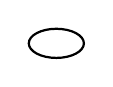
\begin{tikzpicture}
		\draw[thick] (0,0) ellipse (.35cm and .185cm);
	\end{tikzpicture}
	}

\newcommand*{\ansBox}{
	\begin{tikzpicture}
		\draw[thick,fill=readablegreen] (0,0) rectangle (.325,.325);
	\end{tikzpicture}
	}

\newcommand*{\myBox}{ 	
	
\begin{tikzpicture} 		
		\draw[thick] (0,0) rectangle (.325,.325);
	\end{tikzpicture}
	}

%%%%%Answers%%%%%%%%%%%%%%%%%%%%%%%%%%%%%%%%%%%%%%%%%%%%
%%%%%\quest micros set labelitemi for boxes or ovals%%%%
%%Turn answers off/on by uncommenting/commenting renewcommands%%%
\newcommand{\ansE}{\ansEllipse}
\newcommand{\ansB}{\ansBox}
\newcommand{\answer}[1]{\textbf{\textcolor{readablegreen}{#1}}} 
% \renewcommand{\ansE}{\myEllipse}
% \renewcommand{\ansB}{\myBox}
% \renewcommand{\answer}[1]{\textbf{\textcolor{white}{#1}}}

%%%options%%
\renewcommand{\textSize}{\normalsize}
%\tiny \scriptsize \footnotesize \small \normalsize, \large, \Large, \LARGE, \huge, \Huge
\renewcommand{\examTextSize}{\LARGE}
\examTextSize
\renewcommand{\multi}{\cdot}
\renewcommand{\xspace}{\hspace*{0pt}}
%\renewcommand{\yspace}{\vspace{0pt} \newpage} %1.4cm
\begin{enumerate}[resume]
\item \questMulti Which of the following expresses $\frac{5}{16}$ as a
percent?

\begin{itemize}
\item $0.03125\%$
\item $0.3125\%$
\item $3.125\%$
\item [\ansE]$31.25\%$\yspace \vfill
\end{itemize}
\item \questMulti Which of the following is equal to $-2^{2}+2(4-1)^{2}$

\begin{itemize}
\item [\ansE]$14$
\item $22$
\item $32$
\item $45$\yspace \vfill
\end{itemize}
\item \questMulti A two-dimensional net of a certain three-dimensional
figure includes five faces, eight edges, and five vertices. Which
of the following three dimensional figures is represented by the net?

\begin{itemize}
\item Triangular pyramid
\item Triangular prism
\item [\ansE]Rectangular pyramid
\item Rectangular prism\yspace \vfill
\end{itemize}
\item \questMultiPic 
\begin{figure}[H]
\begin{center}
%%%%%%%
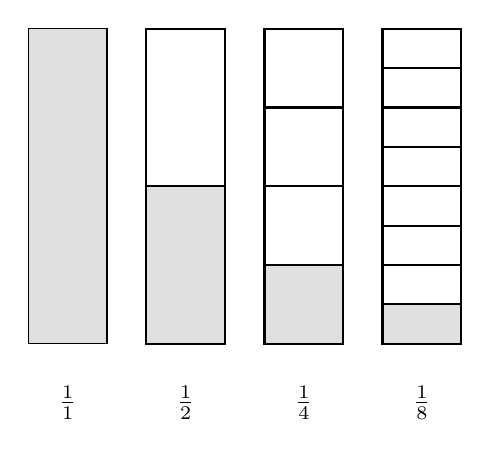
\begin{tikzpicture}[rotate=90]
\def\Height{1.0} \def\Width{4.0} 
\def\Pos{0} \def\Div{1} \def\NodePos{-.75}


%\draw (0,-\Pos) -- (\Width,-\Pos) -- (\Width,\Height- \Pos) 
%	-- (0,\Height- \Pos) -- cycle node[] at (\NodePos,\Height/2) {$\frac{1}{\Div}$};
\def\Pos{0} \def\Div{1}
\draw[fill=gray!25!white] (0,-\Pos) rectangle (\Width/ \Div,\Height-\Pos);
\foreach \x in {1,...,\Div} {
	\draw[black] (0,-\Pos) rectangle (\Width*\x / \Div,\Height-\Pos);
} \node[] at (\NodePos,-\Pos+.5) {$\frac{1}{\Div}$};

\def\Pos{1.5} \def\Div{2}
\draw[fill=gray!25!white] (0,-\Pos) rectangle (\Width/ \Div,\Height-\Pos);
\foreach \x in {1,...,\Div} {
	\draw[thick] (0,-\Pos) rectangle (\Width*\x / \Div,\Height-\Pos);
} \node[] at (\NodePos,-\Pos+.5) {$\frac{1}{\Div}$};

\def\Pos{3} \def\Div{4}
\draw[fill=gray!25!white] (0,-\Pos) rectangle (\Width/ \Div,\Height-\Pos);
\foreach \x in {1,...,\Div} {
	\draw[thick] (0,-\Pos) rectangle (\Width*\x / \Div,\Height-\Pos);
} \node[] at (\NodePos,-\Pos+.5) {$\frac{1}{\Div}$};

\def\Pos{4.5} \def\Div{8}
\draw[fill=gray!25!white] (0,-\Pos) rectangle (\Width/ \Div,\Height-\Pos);
\foreach \x in {1,...,\Div} {
	\draw[thick] (0,-\Pos) rectangle (\Width*\x / \Div,\Height-\Pos);
} \node[] at (\NodePos,-\Pos+.5) {$\frac{1}{\Div}$};

\end{tikzpicture}\end{center}
\end{figure}
\noindent Which of the following is demonstrated by the figure above?

\begin{itemize}
\item When the numerator stays the same and the denominator increases, the
fraction increases.
\item [\ansE]When the numerator stays the same and the denominator increases,
the fraction decreases.
\item When the denominator stays the same and the numerator increases, the
fraction increases.
\item When the denominator stays the same and the numerator increases, the
fraction decreases.\yspace \vfill
\end{itemize}
\item \questMultiPic 
\begin{figure}[H]
\begin{center}%
\begin{tabular}{|c|c|}
\hline 
Week & Customers\tabularnewline
\hline 
1 & 51\tabularnewline
\hline 
2 & 65\tabularnewline
\hline 
3 & 43\tabularnewline
\hline 
4 & 115\tabularnewline
\hline 
5 & 87\tabularnewline
\hline 
6 & 75\tabularnewline
\hline 
7 & 120\tabularnewline
\hline 
8 & 95\tabularnewline
\hline 
9 & 89\tabularnewline
\hline 
\end{tabular}\end{center}
\end{figure}
\noindent A large department store tallies the number of customer
complaints each week for nine consecutive weeks. The number of customer
complaints for each week is shown in the provided table. If the number
of customers who lodged complaints at the store during the tenth week
were included in the data, the mean and median of the data would change
but the range would not change. Which of the following could be the
number of customers complaints during the tenth week?

\begin{itemize}
\item 35
\item 42
\item [\ansE]69
\item 129\yspace \vfill
\end{itemize}
\item \questMultiPic 
\begin{figure}[H]
\begin{center}%
\begin{tabular}{|c|c|c|c|c|}
\hline 
Red & Red & Yellow & Red & Blue\tabularnewline
\hline 
Blue & Green & Red & Blue & Blue\tabularnewline
\hline 
Blue & Green & Yellow & Green & Yellow\tabularnewline
\hline 
Green & Green & Yellow & Green & Green\tabularnewline
\hline 
\end{tabular}\end{center}
\end{figure}
A Pollster asked 20 high-school students to name their favorite color.
The students' responses are shown in the table. \\
\\
The teacher then asked the students to organize and display the data
in a bar graph. Which bar graph correctly displays the data?


\vspace{15pt}
\begin{multicols}{2}
\begin{itemize}
\item %
\begin{minipage}[c][1\totalheight][t]{1\columnwidth}%
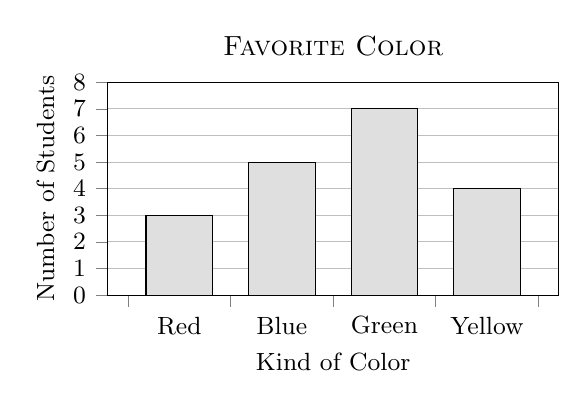
\begin{tikzpicture} 
\begin{axis}[
	scale=.55,
	width=12cm,height=6.5cm,
	title={\textsc{Favorite Color}},
	ymin=0, ymax=8, 
	enlarge x limits=0.05, 
	ybar interval=.65,%%change bar width%% 
	tick align=outside,
	xtick=data,
	ytick={0,1,2,3,...,7,8},
	%y tick label style={/pgf/number format/fixed},
	xticklabel style={text width=35pt, align=center,font=\small},
	yticklabel style={font=\small},
	%scaled y ticks = false,
	%yticklabels={,,},
	%symbolic x coords={0,1,2,3,4,5}, 
	xticklabels={Red,Blue,Green,Yellow},
	xlabel=\small Kind of Color,
	ylabel=\small Number of Students,
	grid=major,
	xmajorgrids=false,
	clip=false, 
	tick pos=left] 	

	\addplot[fill=gray!25!white] coordinates {(1,3) (2,5) (3,7) (4,4) (5,7)} ; 
	%\legend{0-10,10-20,20-30,$>30$} 
\end{axis} 

\end{tikzpicture}%
\end{minipage}
\item %
\begin{minipage}[c][1\totalheight][t]{1\columnwidth}%
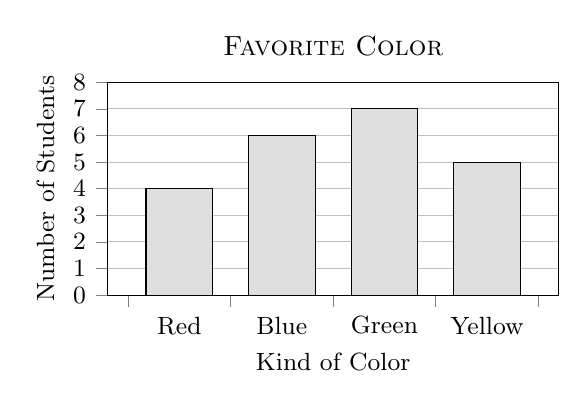
\begin{tikzpicture} 
\begin{axis}[
	scale=.55,
	width=12cm,height=6.5cm,
	title={\textsc{Favorite Color}},
	ymin=0, ymax=8, 
	enlarge x limits=0.05, 
	ybar interval=.65,%%change bar width%% 
	tick align=outside,
	xtick=data,
	ytick={0,1,2,3,...,7,8},
	%y tick label style={/pgf/number format/fixed},
	xticklabel style={text width=35pt, align=center,font=\small},
	yticklabel style={font=\small},
	%scaled y ticks = false,
	%yticklabels={,,},
	%symbolic x coords={0,1,2,3,4,5}, 
	xticklabels={Red,Blue,Green,Yellow},
	xlabel=\small Kind of Color,
	ylabel=\small Number of Students,
	grid=major,
	xmajorgrids=false,
	clip=false, 
	tick pos=left] 	

	\addplot[fill=gray!25!white] coordinates {(1,4) (2,6) (3,7) (4,5) (5,7)} ; 
	%\legend{0-10,10-20,20-30,$>30$} 
\end{axis} 

\end{tikzpicture}%
\end{minipage}
\item [\ansE]%
\begin{minipage}[c][1\totalheight][t]{1\columnwidth}%
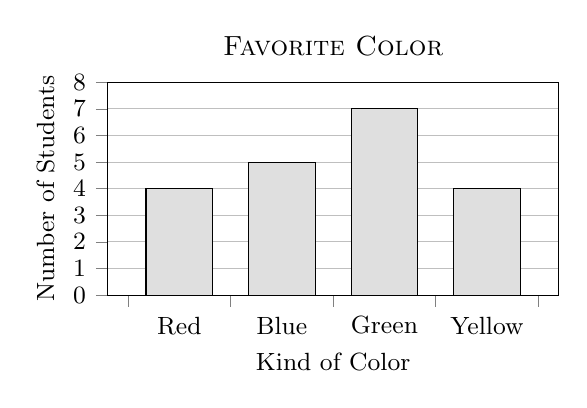
\begin{tikzpicture} 
\begin{axis}[
	scale=.55,
	width=12cm,height=6.5cm,
	title={\textsc{Favorite Color}},
	ymin=0, ymax=8, 
	enlarge x limits=0.05, 
	ybar interval=.65,%%change bar width%% 
	tick align=outside,
	xtick=data,
	ytick={0,1,2,3,...,7,8},
	xticklabel style={text width=35pt, align=center,font=\small},
	yticklabel style={font=\small},
	%scaled y ticks = false,
	%symbolic x coords={0,1,2,3,4,5}, 
	xticklabels={Red,Blue,Green,Yellow},
	xlabel=\small Kind of Color,
	ylabel=\small Number of Students,
	grid=major,
	xmajorgrids=false,
	clip=false, 
	tick pos=left] 	

	\addplot[fill=gray!25!white] coordinates {(1,4) (2,5) (3,7) (4,4) (5,7)} ; 
	%\legend{0-10,10-20,20-30,$>30$} 
\end{axis} 

\end{tikzpicture}%
\end{minipage}
\item %
\begin{minipage}[c][1\totalheight][t]{1\columnwidth}%
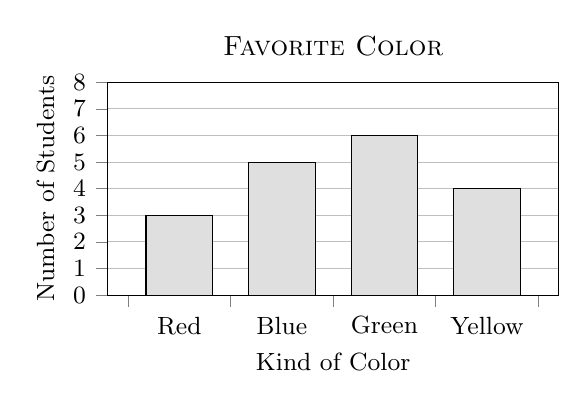
\begin{tikzpicture} 
\begin{axis}[
	scale=.55,
	width=12cm,height=6.5cm,
	title={\textsc{Favorite Color}},
	ymin=0, ymax=8, 
	enlarge x limits=0.05, 
	ybar interval=.65,%%change bar width%% 
	tick align=outside,
	xtick=data,
	ytick={0,1,2,3,...,7,8},
	%y tick label style={/pgf/number format/fixed},
	xticklabel style={text width=35pt, align=center,font=\small},
	yticklabel style={font=\small},
	%scaled y ticks = false,
	%yticklabels={,,},
	%symbolic x coords={0,1,2,3,4,5}, 
	xticklabels={Red,Blue,Green,Yellow},
	xlabel=\small Kind of Color,
	ylabel=\small Number of Students,
	grid=major,
	xmajorgrids=false,
	clip=false, 
	tick pos=left] 	

	\addplot[fill=gray!25!white] coordinates {(1,3) (2,5) (3,6) (4,4) (5,7)} ; 
	%\legend{0-10,10-20,20-30,$>30$} 
\end{axis} 

\end{tikzpicture}%
\end{minipage}
\end{itemize}

\end{multicols}\yspace \vfill

\item \questInd 
\begin{figure}[H]
\begin{center}\renewcommand{\xmin}{-5}
\renewcommand{\xmax}{4}
\renewcommand{\ymin}{-4}
\renewcommand{\ymax}{4}
%%%%%%%
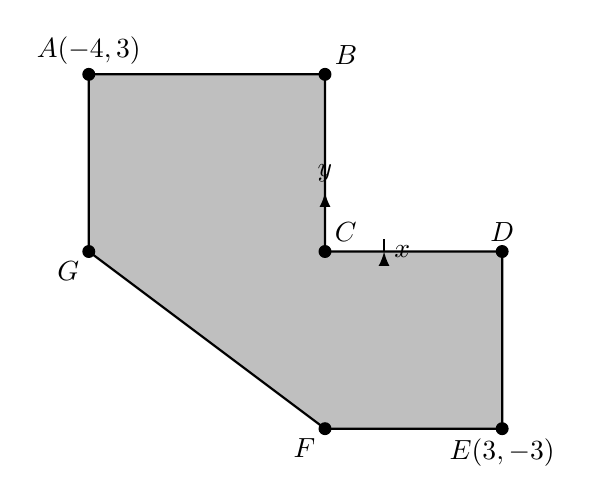
\begin{tikzpicture}[scale=.75]

	\coordinate[label=above:{$A(-4,3)$}] (A) at (-4,3);
	\coordinate[label=above right:{$B$}] (B) at (0,3);
	\coordinate[label=above:{$D$}] (D) at (3,0); %to D
	\coordinate[label=below:{$E(3,-3)$}] (E) at (3,-3); %to E			
	\coordinate[label=below left:{$F$}] (F) at (0,-3);	%to F
	\coordinate[label=above right:{$C$}] (C) at (0,0); %to C
	\coordinate[label=below left:{$G$}] (G) at (-4,0);	
	
	\draw[thick,fill=gray!50!white] (A)--(B)--(C)--(D)--(E)--(F)--(G)--cycle;
	\foreach \x in {A,B,C,D,E,F,G} {
		\draw[fill=black] (\x) circle (0.1);
		}
	
	\draw[-latex,thick](\xmin,0)--(\xmax,0) node[anchor=west]{$x$};
	\draw[-latex,thick](0,\ymin)--(0,\ymax) node[anchor=south]{$y$};

\end{tikzpicture}\end{center}
\end{figure}

\noindent In the figure shown, the quadrilateral $ABCG$ is a rectangle
and the quadrilateral $CDEF$ is a square. Which of the following
statements must be true about the figure?\\
\\
Select \textbf{all }that apply.

\begin{itemize}
\item[\ansBox] $F$ lies on the y -axis.
\item $B$ lies on the $x$-axis.
\item $A$ is in the first quadrant.
\item[\ansBox] $E$ is in the fourth quadrant
\item[\ansBox] The area of the polygon $ABCDEFG$ is 27 square units.
\item The perimeter of the polygon $ABCDEFG$ is 23 units.\yspace \vfill
\end{itemize}

\item \questMulti Which of the following is equal to $2(100^{0})$?

\begin{itemize}
\item 0
\item 1
\item [\ansE]2
\item 200\yspace \vfill
\end{itemize}
\item \questMulti A pencil is 21 centimeters in length. How long is the
pencil in millimeters?

\begin{itemize}
\item $0.21$
\item $2.1$
\item [\ansE]$210$
\item $2,100$\yspace \vfill
\end{itemize}
\item \questMulti If the geometric sequence below continues to increase
in the same way, what is the next number in the sequence?
\[
3,9,27,81,243\dots
\]


\begin{itemize}
\item 324
\item 486
\item [\ansE]729
\item 972\yspace \vfill
\end{itemize}
\item \questMulti Which of the following lists the coefficients and degrees
of the terms in the polynomial shown?
\[
4x^{6}+7x^{4}-6
\]


\begin{itemize}
\item [\ansE]Coefficients: $4,7,-6$; Degrees: $6,4,0$
\item Coefficients: $4,7,-6$; Degrees: $6,4,1$
\item Coefficients: $2,4,0$; Degrees: $4,7,-6$
\item Coefficients: $2,4,1$; Degrees: $4,7,-6$\yspace \vfill
\end{itemize}
\item \questMulti In which quadrant is the point $(5,-2)$ located? 

\begin{itemize}
\item Quadrant I
\item Quadrant II
\item Quadrant III
\item [\ansE]Quadrant IV\yspace \vfill
\end{itemize}
\item \questMultiPic 
\begin{figure}[H]
\begin{center}\begin{tabular}{|c|} 
	\hline  
	Edwins's number: $15,293,863$\rule{0pt}{2.6ex}\rule[-0.9ex]{0pt}{0pt}
	\tabularnewline 
	\hline
	\noalign{\vskip 5pt}  
	\hline  
	Tess's number: $29,018,335$\rule{0pt}{2.6ex}\rule[-0.9ex]{0pt}{0pt}
	\tabularnewline 
	\hline  
\end{tabular}\end{center}
\end{figure}
\noindent Both Edwin and Tess wrote a number, as shown above. The
digit 9 in Tess's number represents how many times what digit 9 represents
in Edwin's number?

\begin{itemize}
\item [\ansE]100
\item 1,000
\item 10,000
\item 1,000,000\yspace \vfill
\end{itemize}
\item \questMultiPic 
\begin{figure}[H]
\begin{center}$4z+2z$\end{center}
\end{figure}
What is the value of the algebraic expression shown when $z=3$

\begin{itemize}
\item 12
\item [\ansE]18
\item 21
\item 87\yspace \vfill
\end{itemize}
\item \questMultiPic 
\begin{figure}[H]
\begin{center}\begin{tikzpicture}[scale=.85]
	\def\BigL{8}
	\def\BigH{7}
	\def\LitL{5}
	\def\LitH{3}

	\coordinate (A) at (0,0);%%Bg rectangle pts
	\coordinate (A1) at (0,\BigH/2-\LitH/2); %%intersection pts
	\coordinate (A2) at (\BigL/2-\LitL/2,\BigH/2-\LitH/2);
	\coordinate (B) at (\BigL,0);
	\coordinate (B1) at (\BigL,\BigH/2-\LitH/2);
	\coordinate (B2) at (\BigL+\LitL/2-\BigL/2,\BigH/2-\LitH/2);
	\coordinate (C) at (\BigL,\BigH);
	\coordinate (C1) at (\BigL,\BigH/2+\LitH/2);
	\coordinate (C2) at (\BigL+\LitL/2-\BigL/2,\BigH/2+\LitH/2);
	\coordinate (D) at (0,\BigH);
	\coordinate (D1) at (0,\BigH/2+\LitH/2);
	\coordinate (D2) at (\BigL/2-\LitL/2,\BigH/2+\LitH/2);

	%\path let \p1 = (A) in coordinate (A1) at (2*\x1,\y1/2);
	
	\draw[thick] (A)
	--(B)
	--(B1)
	--(B2) 
	--(C2)
	--(C1)
	--(C) 
	--(D)
	--(D1)
	--(D2)
	--(A2)
	--(A1)
	--(A)
	--cycle;
	%\tkzLabelPoints[below left](A,A1,A2,B,B1,B2,C,C1,C2,D,D1,D2)
	\tkzMarkRightAngle[size=0.35,opacity=1](D,A,B) 
	\tkzMarkRightAngle[size=0.35,opacity=1](A,B,C)
	%\tkzMarkRightAngle[size=0.35,opacity=1](B1,B2,C2)
	%\tkzMarkRightAngle[size=0.35,opacity=1](B2,C2,C1)
	\tkzMarkRightAngle[size=0.35,opacity=1](C1,C,D)
	\tkzMarkRightAngle[size=0.35,opacity=1](C,D,D1)
	%\tkzMarkRightAngle[size=0.35,opacity=1](D1,D2,A2)
	%\tkzMarkRightAngle[size=0.35,opacity=1](D2,A2,A1)
	\tkzMarkRightAngle[size=0.35,opacity=1](A,A1,A2)
	\tkzMarkRightAngle[size=0.35,opacity=1](B,B1,B2)
	\tkzMarkRightAngle[size=0.35,opacity=1](C,C1,C2)
	\tkzMarkRightAngle[size=0.35,opacity=1](D,D1,D2)		

	%\tkzLabelSegment[below=1pt](A,B){$10$} 
	%\tkzLabelSegment[right=1pt](B,C){$10$} 
	%\tkzLabelSegment[left=1pt](C,A){$$}
	%\node at (1.4,.4) {\small $A=\frac{1}{2}bh$};
	%\tkzLabelPoints[below right](B)
	%\tkzLabelPoints[above right](C)	

	%\tkzMarkRightAngle[](C,B,A) 
	%\tkzLabelAngle[pos = 0.6](C,B,A){$\alpha$}

	%\tkzMarkAngle[size=0.7cm, opacity=1.0](A,C,B) 	%\tkzLabelAngle[pos = 0.5](A,C,B){$65$}

\end{tikzpicture} \end{center}
\end{figure}
Which of the following could be used to describe the polygon shown

\begin{itemize}
\item Regular and convex
\item Regular and concave
\item Irregular and convex
\item [\ansE]Irregular and concave\yspace \vfill
\end{itemize}
\item \questMultiPic  
\begin{figure}[H]
\begin{center}%
\fbox{\begin{minipage}[t]{0.55\textwidth}%
Stephen went to the grocery store to buy some food. He bought eight
vegetables, half as many fruits as vegetables, and a third as many
cans of soup as vegetables. How many items did Stephen buy? %
\end{minipage}} \end{center}
\end{figure}
\noindent Which of the following statements about the solution to
the word problem shown must be true?

\begin{itemize}
\item Because of the real-world context, the solution must belong to the
set of all rational positive numbers; therefore the solution is acceptable.
\item Because of the real-world context, the solution must belong to the
set of all rational positive numbers; therefore the solution is not
acceptable.
\item Because of the real-world context, the solution must belong to the
set of all natural numbers; therefore the solution is acceptable.
\item [\ansE]Because of the real-world context, the solution must belong
to the set of all natural numbers; therefore the solution is not acceptable.\yspace \vfill
\end{itemize}
\item \questMulti Which of the following graphs in the $xy$-plane could
be used to solve graphically the inequality $-x+2>2(x+1)$ and shows
the solution to the inequality?


\vspace{15pt}
\begin{multicols}{2}
\begin{itemize}
\item %
\begin{minipage}[c][1\totalheight][t]{1\columnwidth}%
\renewcommand{\xmin}{-5} 
\renewcommand{\xmax}{5} 
\renewcommand{\ymin}{-5} 
\renewcommand{\ymax}{5} 
%%%%%%%
\begin{tikzpicture}
\begin{axis}[height=6cm, 
	width=6cm, 
	axis lines=middle,
	minor x tick num={1},
	minor y tick num={1},
	grid=none,ticks=major,
	xmin=\xmin,xmax=\xmax, 
	ymin=\ymin,ymax=\ymax,
	%xtick={-4,-3,-2,-1,0,1,2,3,4}, 
	%ytick={-4,-3,-2,-1,0,1,2,3,4},
	%xticklabels={},
	%yticklabels={},
	axis line style={-latex}, 
	%restrict y to domain=-1:10,
	%no markers, 
	%every axis x label/.append style={anchor=west}, 
	%every axis y label/.append style={anchor=south},
	%x label style={at={(axis description cs:0.5,-0.0)},anchor=north},     
	%y label style={at={(axis description cs:-0.0,0.5)},rotate=90,anchor=south},
	%xlabel={\small Time Studying},
	%ylabel={\small Test Score},
	%clip=false, %doesn't clip outside graph
	]
	
	\addplot[domain=\xmin-11:\xmax+1,samples=2,draw=black,thick,latex-latex]{-x+2} [yshift=5pt] node[pos=0.5,above] {$$};
	\addplot[domain=\xmin-11:\xmax+1,samples=2,draw=black,thick,latex-latex]{2*x+2)} [yshift=5pt] node[pos=0.5,above] {$$};
	\addplot[domain=0:\xmax+1,samples=2,draw=black,ultra thick]{-x+2};
	
	\node[anchor=west] at (axis cs:\xmax,0) {$x$}; 
	\node[anchor=south] at (axis cs:0,\ymax) {$y$};

\end{axis}
\end{tikzpicture}%
\end{minipage}

\begin{itemize}
\item []
\end{itemize}
\item %
\begin{minipage}[c][1\totalheight][t]{1\columnwidth}%
\renewcommand{\xmin}{-5} 
\renewcommand{\xmax}{5} 
\renewcommand{\ymin}{-5} 
\renewcommand{\ymax}{5} 
%%%%%%%
\begin{tikzpicture}
\begin{axis}[height=6cm, 
	width=6cm, 
	axis lines=middle,
	minor x tick num={1},
	minor y tick num={1},
	grid=none,ticks=major,
	xmin=\xmin,xmax=\xmax, 
	ymin=\ymin,ymax=\ymax,
	%xtick={-4,-3,-2,-1,0,1,2,3,4}, 
	%ytick={-4,-3,-2,-1,0,1,2,3,4},
	%xticklabels={},
	%yticklabels={},
	axis line style={-latex}, 
	%restrict y to domain=-1:10,
	%no markers, 
	%every axis x label/.append style={anchor=west}, 
	%every axis y label/.append style={anchor=south},
	%x label style={at={(axis description cs:0.5,-0.0)},anchor=north},     
	%y label style={at={(axis description cs:-0.0,0.5)},rotate=90,anchor=south},
	%xlabel={\small Time Studying},
	%ylabel={\small Test Score},
	%clip=false, %doesn't clip outside graph
	]
	
	\addplot[domain=\xmin-11:\xmax+1,samples=2,draw=black,thick,latex-latex]{-x+2} [yshift=5pt] node[pos=0.5,above] {$$};
	\addplot[domain=\xmin-11:\xmax+1,samples=2,draw=black,thick,latex-latex]{2*x+2)} [yshift=5pt] node[pos=0.5,above] {$$};
	\draw[ultra thick] (0,2)--(0,5);
	
	\node[anchor=west] at (axis cs:\xmax,0) {$x$}; 
	\node[anchor=south] at (axis cs:0,\ymax) {$y$};

\end{axis}
\end{tikzpicture}%
\end{minipage}

\begin{itemize}
\item []
\end{itemize}
\item [\ansE]%
\begin{minipage}[c][1\totalheight][t]{1\columnwidth}%
\renewcommand{\xmin}{-5} 
\renewcommand{\xmax}{5} 
\renewcommand{\ymin}{-5} 
\renewcommand{\ymax}{5} 
%%%%%%%
\begin{tikzpicture}
\begin{axis}[height=6cm, 
	width=6cm, 
	axis lines=middle,
	minor x tick num={1},
	minor y tick num={1},
	grid=none,ticks=major,
	xmin=\xmin,xmax=\xmax, 
	ymin=\ymin,ymax=\ymax,
	%xtick={-4,-3,-2,-1,0,1,2,3,4}, 
	%ytick={-4,-3,-2,-1,0,1,2,3,4},
	%xticklabels={},
	%yticklabels={},
	axis line style={-latex}, 
	%restrict y to domain=-1:10,
	%no markers, 
	%every axis x label/.append style={anchor=west}, 
	%every axis y label/.append style={anchor=south},
	%x label style={at={(axis description cs:0.5,-0.0)},anchor=north},     
	%y label style={at={(axis description cs:-0.0,0.5)},rotate=90,anchor=south},
	%xlabel={\small Time Studying},
	%ylabel={\small Test Score},
	%clip=false, %doesn't clip outside graph
	]
	
	\addplot[domain=\xmin-1:\xmax+1,samples=2,draw=black,thick,latex-latex]{-x+2} [yshift=5pt] node[pos=0.5,above] {$$};
	\addplot[domain=\xmin-1:\xmax+1,samples=2,draw=black,thick,latex-latex]{2*x+2)} [yshift=5pt] node[pos=0.5,above] {$$};
	\addplot[domain=\xmin-1:0,samples=2,draw=black,ultra thick]{0};
	
	\node[anchor=west] at (axis cs:\xmax,0) {$x$}; 
	\node[anchor=south] at (axis cs:0,\ymax) {$y$};

\end{axis}
\end{tikzpicture}%
\end{minipage}

\begin{itemize}
\item []
\end{itemize}
\item %
\begin{minipage}[c][1\totalheight][t]{1\columnwidth}%
\renewcommand{\xmin}{-5} 
\renewcommand{\xmax}{5} 
\renewcommand{\ymin}{-5} 
\renewcommand{\ymax}{5} 
%%%%%%%
\begin{tikzpicture}
\begin{axis}[height=6cm, 
	width=6cm, 
	axis lines=middle,
	minor x tick num={1},
	minor y tick num={1},
	grid=none,ticks=major,
	xmin=\xmin,xmax=\xmax, 
	ymin=\ymin,ymax=\ymax,
	%xtick={-4,-3,-2,-1,0,1,2,3,4}, 
	%ytick={-4,-3,-2,-1,0,1,2,3,4},
	%xticklabels={},
	%yticklabels={},
	axis line style={-latex}, 
	%restrict y to domain=-1:10,
	%no markers, 
	%every axis x label/.append style={anchor=west}, 
	%every axis y label/.append style={anchor=south},
	%x label style={at={(axis description cs:0.5,-0.0)},anchor=north},     
	%y label style={at={(axis description cs:-0.0,0.5)},rotate=90,anchor=south},
	%xlabel={\small Time Studying},
	%ylabel={\small Test Score},
	%clip=false, %doesn't clip outside graph
	]
	
	\addplot[domain=\xmin-1:\xmax+1,samples=2,draw=black,thick,latex-latex]{-x+2} [yshift=5pt] node[pos=0.5,above] {$$};
	\addplot[domain=\xmin-1:\xmax+1,samples=2,draw=black,thick,latex-latex]{2*x+2)} [yshift=5pt] node[pos=0.5,above] {$$};
	\addplot[domain=\xmin-1:\xmax+1,samples=2,draw=black,ultra thick]{-x+2};
	
	\node[anchor=west] at (axis cs:\xmax,0) {$x$}; 
	\node[anchor=south] at (axis cs:0,\ymax) {$y$};

\end{axis}
\end{tikzpicture}%
\end{minipage}
\end{itemize}

\end{multicols}\yspace \vfill

\item \questMulti Mrs.~Smith gave her students the following table and
asked them to determine function rules for the provided data.
\begin{figure}[H]
\begin{center}%
\begin{tabular}{|c|c|}
\hline 
$x$ & $y$\tabularnewline
\hline 
-1 & 1\tabularnewline
\hline 
0 & 0\tabularnewline
\hline 
\end{tabular}\end{center}
\end{figure}
Adeline says the function rule is $y=-x^{3}$, Brent says that the
function rule is $y=-x$, and Chad says that the function rule is
$y=-x^{2}-2x$. Which of the three equations could be the function
rule for the table?

\begin{itemize}
\item only Brent's
\item only Brent's and Adeline's
\item only Brent's and Chad's
\item [\ansE]Brent's, Adeline's, and Chad's\yspace \vfill
\end{itemize}
\item \questMulti A public fountain holds of 42,300 liters of water. A
crack is leaking at a rate of 75 liters per hour. The equation $\ell=42,300-75h$
can be used to find the number of liters $\ell$ remaining in the
fountain after $h$ days. Which of the following statements is true?

\begin{itemize}
\item $\ell$ is the independent variable because it is what needs to be
found.
\item [\ansE]$\ell$ is the dependent variable because the volume is dependent
on the number of hours $h$.
\item $h$ is the dependent variable because it is being multiplied by the
independent rate of $-75$.
\item Dependent and independent varaiables cannot be determined in this
situation because the equation is linear.\yspace \vfill
\end{itemize}
\item \questFill Tiana needs to pack 1,120 candies into boxes. If a box
can hold 350 candies, how many boxes does she need to pack all the
candies. 
\[
\fbox{{\ensuremath{\begin{array}{cc}
 \,  &  \answer{4} \,\,\end{array}}}}
\]
\yspace \vfill
\item \questMulti In the number $756,814$ what is the value of the digit
5?

\begin{itemize}
\item Fifty
\item Five thousand
\item Ten thousand
\item [\ansE]Fifty thousand\yspace \vfill
\end{itemize}
\item \questMulti Kathryn setup a saving's account by making an initial
deposit of \$120. Each month, Kathryn deposits \$24 into the savings
account. The amount of money she has saved after $x$ weeks can be
represented with the expression $24x+120$. This expression is equivalent
to which of the following expressions? 

\begin{itemize}
\item $4(6x+120)$
\item $4(6x+20)$
\item [\ansE]$6(4x+20)$
\item $6(4x+100)$\yspace \vfill
\end{itemize}
\item \questMultiPic 
\begin{figure}[H]
\begin{center}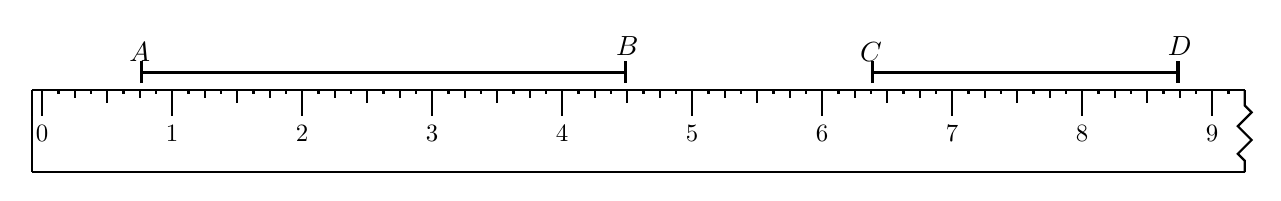
\begin{tikzpicture}[scale=.65]
	\def\inches{9.25}            
	\def\L{23.495} %measuring length
	\def\RH{1.6} %ruler height
	\def\RL{\L} %ruler length
	\draw[thick] (-0.2,0)--(\RL,0) node[pos=.5,above] {};
	\draw[thick,decoration={zigzag}] (\RL,0)-- (\RL,.22) decorate {--(\RL,\RH-.22)}--(\RL,\RH);
	\draw[thick] (\RL,\RH)--(-0.2,\RH);
	\draw[thick] (-0.2,\RH)--(-0.2,0);
%% lower divisions centimeters; ratio is approx L=1 to 2.54            
	%\foreach \x in {0,1,...,\L}{             
	%	\draw (\x,0) -- (\x,0.2)node[above,scale=0.4]{\x};             
	%}             
	%\foreach \x in {0.1,0.2,...,\L-.1}{             
	%	\draw (\x,0) -- (\x,0.075);             
	%}             
	%\foreach \x in {0.5,1,...,\L-.5}{             
	%	\draw (\x,0) -- (\x,0.15);             
	%}             
% Upper divisions inches            
	\foreach \x in {0,1,...,\inches}{             
		\draw[thick] (\x in,\RH) -- (\x in,\RH-.5)node[below,scale=.9]{\x};             
	}             
	\foreach \x in {0.5,1,...,\inches}{             
		\draw[thick] (\x in,\RH) -- (\x in,\RH-.25);             
	}             
	\foreach \x in {0.25,0.5,...,\inches}{          
		\draw[thick] (\x in,\RH) -- (\x in,\RH-.15);             
	}
	\foreach \x in {0.125,0.25,...,\inches}{          
		\draw[thick] (\x in,\RH) -- (\x in,\RH-.075);             
	}
%%lines above ruler%%
	\draw[|-|,very thick] (.75*2.54,\RH+.35) node[above]{$A$} -- (4.5*2.54,\RH+.35) node[above, yshift=2pt]{$B$};
	\draw[|-|,very thick] (6.375*2.54,\RH+.35) node[above]{$C$} -- (8.75*2.54,\RH+.35) node[above, yshift=2pt]{$D$};
     
\end{tikzpicture}\end{center}\caption*{\textbf{\uline{Note}}: Figure not drawn
to scale} 
\end{figure}
\noindent The figure shows a ruler with inches marked and \uline{two}
line segments drawn. To the nearest eight of an inch, how much longer,
in inches, is the length of $\overline{AB}$ than the length of $\overline{CD}$?

\begin{itemize}
\item [\ansE]$1\frac{3}{8}$
\item $1\frac{1}{2}$
\item $1\frac{5}{8}$
\item 2
\item $3.75$\yspace \vfill
\end{itemize}
\item \questMulti Which of the following numbers is the greatest?

\begin{itemize}
\item 0.1031
\item 0.1004
\item [\ansE]0.105
\item 0.10009\yspace \vfill
\end{itemize}
\item \questMulti In February, 20 percent of the 3750 students at a high
schools had a perfect attendance record. Which of the following computations
can be used to determine the number of students with a perfect attendance
record?

\begin{itemize}
\item $20\times\mbox{3,750}$
\item $\frac{20}{\mbox{3,750}}$
\item $\frac{1}{20}\times\mbox{3,750}$
\item [\ansE]$\frac{1}{5}\times\mbox{3,750}$\yspace \vfill
\end{itemize}
\item \questMulti In the formula, $d=r\times t$, if $d$ equals 75 and
$t$ remains constant, which of the following is equivalent to $r$?

\begin{itemize}
\item $75t$
\item [\ansE]$\frac{75}{t}$
\item $\frac{t}{75}$
\item $\frac{d}{75t}$\yspace \vfill
\end{itemize}
\item \questMultiPic 
\begin{figure}[H]
\begin{center}$17(4-7)=17\times4-17\times7$\end{center}
\end{figure}
\noindent The equation shown demonstrates which of the following?

\begin{itemize}
\item [\ansE]The distributive property of multiplication over addition.
\item The commutative property of multiplication.
\item The associative property of multiplication.
\item The additive inverse and additive identity properties.\yspace \vfill
\end{itemize}
\item \questMulti Which of the following is the product of two odd numbers
and an even number, each of which is greater than 1?

\begin{itemize}
\item 16
\item 24
\item 27
\item [\ansE]30\yspace \vfill
\end{itemize}
\item \questMulti A pet food company makes 12-kilogram and 30-kilogram
bags of dog food. For the 12-kilogram bag, the company uses 5-kilograms
of chicken meat, and the rest is corn. If the proportion of chicken
meat is the same in the 30-kilogram bag as the 12-kilogram bag, how
many kilograms of corn does the 30-kilogram bag have?

\begin{itemize}
\item $2.8$
\item $12.5$
\item [\ansE]$17.5$
\item 20\yspace \vfill
\end{itemize}
\item \questMultiPic
\begin{figure}[H]
\begin{center}%
\begin{tabular}{rl}
Step 1: & Select a numerical value for the variable $b$.\tabularnewline
Step 2: & Add 5 to $b$.\tabularnewline
Step 3: & Multiply the result by $2$.\tabularnewline
Step 4: & Square the result.\tabularnewline
Step 5: & End\tabularnewline
\end{tabular}\end{center}
\end{figure}
\noindent Consider the algorithm shown above. Following the algorithm
is equivalent to evaluating which of the following algebraic expressions?

\begin{itemize}
\item $(2b+5)^{2}$
\item $2(b+5)^{2}$
\item $2^{2}(b+5)$
\item [\ansE]$2^{2}(b+5)^{2}$\yspace \vfill
\end{itemize}
\item \questMulti The first two terms of the sequence shown are 3 and 4.
Each subsequent term, beginning with the third, is found by adding
the two preceding terms and multiplying the sum by $-2$. What is
$n_{5}$, the fifth term of the sequence?
\[
3,4,n_{3},n_{4},n_{5},\dots
\]


\begin{itemize}
\item $-16$
\item $-14$
\item [\ansE]$-12$
\item $-10$\yspace \vfill
\end{itemize}
\item \questInd 
\begin{figure}[H]
\begin{center}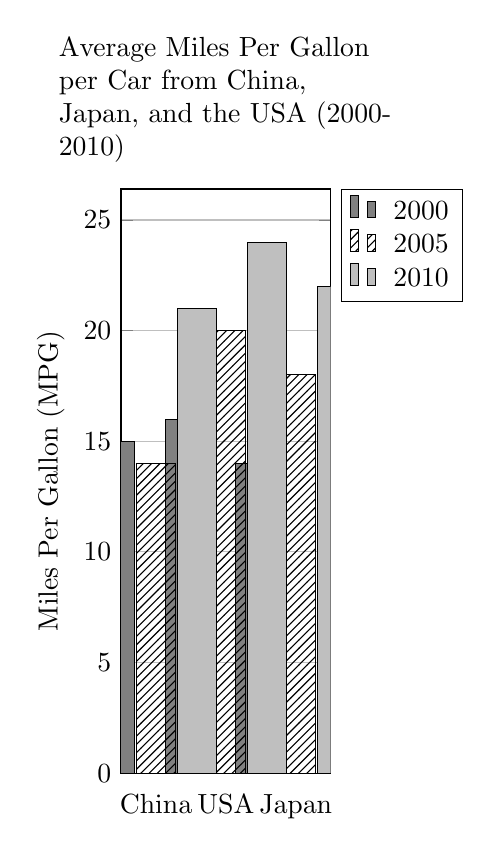
\begin{tikzpicture}     
\begin{axis}[         
	width  = 0.35*\textwidth,         
	height = 9cm,         
	major x tick style = transparent,         
	ybar=2*\pgflinewidth,         
	bar width=14pt,         
	ymajorgrids = true,         
	title style = {text width=.35*\textwidth},
	title  = {Average Miles Per Gallon per Car from China, Japan, and the USA (2000-2010)},
	ylabel = {Miles Per Gallon (MPG)},         
	symbolic x coords={China, USA, Japan},         
	xtick = data,         
	scaled y ticks = false,         
	enlarge x limits=0.25,         
	ymin=0,         
	legend cell align=left,         
	legend style={
		at={(1.05,1)},                 
		anchor=north west ,                 
		column sep=1ex         
		}     
	]         
	%%Suv
	\addplot[style={black,fill=black!50!white,mark=none}]             
		coordinates {(China, 15) (USA,16) (Japan,14)};
    %%Sedan    
	\addplot[pattern=north east lines,pattern color=black]              
		coordinates {(China, 14) (USA,20) (Japan,18)};
    %%Sports    
	\addplot[style={black,fill=black!25!white,mark=none}]              
		coordinates {(China, 21) (USA,24) (Japan,22)};
        
    \legend{2000, 2005, 2010}     
\end{axis} 
\end{tikzpicture}\end{center}
\end{figure}
\noindent Which of the following statements can be inferred from
the graph shown?

\begin{itemize}
\item For each country, the average MPG increased each year from the previous
year
\item [\ansB]The country that had the greatest yearly average MPG for each
of the three years shown had a three year total between 55 and 65
MPG.
\item [\ansB]The average MPG in China increase by more than one third from
2000 to 2010.
\item The average MPG in the USA in 2010 was more than double of that in
China in 2000.\yspace \vfill
\end{itemize}
\item \questMultiPic 
\begin{figure}[H]
\begin{center}%
\begin{tabular}{|c|c|}
\hline 
$x$ & $f(x)$\tabularnewline
\hline 
60 & \tabularnewline
\hline 
25 & -5\tabularnewline
\hline 
20 & -2\tabularnewline
\hline 
15 & 1\tabularnewline
\hline 
\end{tabular}\end{center}
\end{figure}
\noindent Values of the linear function $f$ are provided in the
table shown. Find $f(60)$.

\begin{itemize}
\item $-8$
\item $-14$
\item $-20$
\item [\ansE]$-26$\yspace \vfill
\end{itemize}
\item \questMulti Wei tossed a fair coin 12 times with an outcome of $H,T,H,T,T,T,H,H,T,T,T,T$,
where $H$ means the coin landed on heads and $T$ means the coin
landed on $H$. Approximately what is the probability that the next
toss will be $T$?

\begin{itemize}
\item $0.67$
\item [\ansE]$0.5$
\item $0.33$
\item $0.83$\yspace \vfill
\end{itemize}
\item \questMultiPic 
\begin{figure}[H]
\begin{center}%%draw regular polygon
%%requires \usepackage{luamplib}%%%	
%\begin{mplibcode}   
	%beginfig(1);     
	%u = 3cm; n = 5; angl = 360/n;     
	%% The regular polygon at the center     
	%z0 = u*dir(-90 - .5angl);     
	%path polygon;      
	%polygon = z0 for i = 1 upto n-1: hide(z[i] = z[i-1] rotated angl) -- z[i] endfor -- cycle;     
	%% Drawing the other polygons 
	%for i = 0 upto n-1: draw polygon rotatedaround (z[i], 180-angl); 
	%endfor;   
	%endfig; 
%\end{mplibcode}

%%%using tikz%%%%
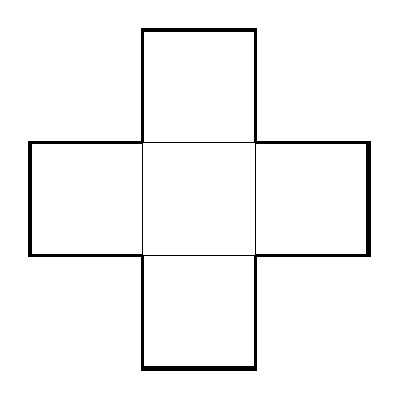
\begin{tikzpicture}[scale=2.2]   

%thick outside
\tikzset{pntgn/.style={regular polygon, regular polygon sides=4,draw,ultra thick,minimum size=2cm,anchor=south}}   
	\node(n)[pntgn,draw=none,outer sep=0pt]{};   
	\foreach\deg[count=\x] in{0,90,...,270}{\node[pntgn,rotate=\deg,at=(n.side \x)]{};}
%thin inside
\tikzset{pntgn/.style={fill=white,regular polygon, regular polygon sides=4,draw, minimum size=2cm,anchor=south}}   
	\node(n)[pntgn,draw=none,outer sep=0pt]{};   
	\foreach\deg[count=\x] in{0,90,...,270}{\node[pntgn,rotate=\deg,at=(n.side \x)]{};} %%node at end
	%..\foreach list should be {0,60,...,300} instead, because 
	%side 1 corresponds to rotation=0, side 2 to rotation=60, ... and side 6 to rotation=300
	%example pentagons= \foreach\deg[count=\x] in{36,108,...,324}
\end{tikzpicture}\end{center}
\end{figure}
\noindent If the perimeter of each of the five regular quadrilaterals
in the figure shown is 24, what is the perimeter of the figure?

\begin{itemize}
\item [\ansE]72
\item 84
\item 120
\item 144\yspace \vfill
\end{itemize}
\item \questMulti The population of a certain county was 200,000 people.
Ten years later the population of the same county had decreased to
192,000. Approximately, what was the percent decrease in the county's
population in that ten year period?

\begin{itemize}
\item [\ansE]4\%
\item 4.17\%
\item 40\%
\item 41.7\%\yspace \vfill
\end{itemize}
\item \questMulti Which of the following is an example of the associative
property of addition? 

\begin{itemize}
\item $(a+b)+c=(b+a)+c$
\item $ab+c=ba+c$
\item [\ansE]$(a+b)+c=a+(b+c)$
\item $a(b+c)=ab+ac$\yspace \vfill
\end{itemize}
\item \questMulti What is the greatest odd factor of 1,344?

\begin{itemize}
\item $3$
\item $7$
\item [\ansE]$21$
\item $113$\yspace \vfill
\end{itemize}
\item \questMulti At a school bake sale, Ted sold pies for \$5.00 each
and cookies for \$1.50 each. Nancy spent a total of \$16.50 on Ted's
pies and cookies. If Nancy bought at least one cookie and one pie,
how many pies did she buy?

\begin{itemize}
\item 1
\item 2
\item [\ansE]3
\item 4\yspace \vfill
\end{itemize}
\item \questMulti The Carolina Panthers football team scored an average
of $35$ points in 5 games. In the first four games, the team scored
28, 34, 35, and 40 points. How many points did they score in their
fifth game?

\begin{itemize}
\item 30
\item 36
\item 37
\item [\ansE]38\yspace \vfill
\end{itemize}
\item \questMulti On Gwen's map, 30 miles is represented by 1 inch, and
on Luke's map, 40 miles is represented by 1 inch. The area represented
by a 1-inch by 1-inch square is how many more square miles on Luke's
map than on Gwen's map?

\begin{itemize}
\item 10
\item [\ansE]700
\item 1600
\item 2500\yspace \vfill
\end{itemize}
\item \questInd Which of the following are equivalent to dividing 306 by
18\\
\\
Select \textbf{all }that apply.

\begin{itemize}
\item [\ansB]$(306\div2)\div9$
\item [\ansB]$2(153\div18)$
\item $(153\div9)+(153\div9)$
\item [\ansB]$(260\div18)+(46\div18)$\yspace \vfill
\end{itemize}
\item \questMultiPic 
\begin{figure}[H]
\begin{center}%
\begin{tabular}{|c|c|}
\hline 
\textbf{Item} & \textbf{Cost}\tabularnewline
\hline 
Hammer & \$5.53\tabularnewline
\hline 
Nails & \$5.09\tabularnewline
\hline 
Bucket & \$5.99\tabularnewline
\hline 
Brush & \$5.09\tabularnewline
\hline 
Pencil & \$1.79\tabularnewline
\hline 
Washers & \$5.29\tabularnewline
\hline 
\end{tabular}\end{center}\caption*{Prices include sales tax}
\end{figure}
\noindent Joe goes to the hardware store and purchases one of each
item in the list above at the indicated prices. If Joe pays with two
\$20 bills, which of the following is closest to the change he would
receive? 

\begin{itemize}
\item [\ansE]\$11
\item \$12
\item \$13
\item \$14\yspace \vfill
\end{itemize}
\item \questMulti Which of the following has the greatest value?

\begin{itemize}
\item 7,200 ones
\item 708 tens
\item [\ansE]73 hundreds
\item 7 thousands\yspace \vfill
\end{itemize}
\item \questMulti A flag pole casts a shadow that is 23 feet long. Nearby,
a stop sign with a height of 7 feet casts a shadow that is 3 feet
long. Assuming that flag pole and stop sign are both perpendicular
to the ground, the height of the flag pole must be between which of
the following values? 

\begin{itemize}
\item 0 and 10 feet
\item 40 and 50 feet
\item [\ansE]50 and 60 feet
\item 170 and 180 feet\yspace \vfill
\end{itemize}
\item \questMulti Bonnie's night work shift began at $7:53$ \textsc{p.m.}~and
ended at $5:29$ \textsc{a.m.} How long did her shift last?

\begin{itemize}
\item 8 hours and 22
\item 8 hours and 36 minutes
\item 9 hours and 22 minutes
\item [\ansE]9 hours and 36 minutes\yspace \vfill
\end{itemize}
\item \questMulti Suppose that it takes 3 hours to mow an acre of grass.
Which of the following expression represents the number of acres that
can be mowed in $h$ hours.

\begin{itemize}
\item 3$h$
\item [\ansE]$\frac{h}{3}$
\item $\frac{h}{60\times3}$
\item $\frac{60\times h}{3}$\yspace \vfill
\end{itemize}
\item \questMultiPic 
\begin{figure}[H]
\begin{center}%
\begin{tabular}{|c|c|}
\hline 
\hspace{1cm}$x$\hspace{1cm} & \hspace{1cm}$y$\hspace{1cm}~\tabularnewline
\hline 
$-20$ & $-10$\tabularnewline
\hline 
$-10$ & $0$\tabularnewline
\hline 
$10$ & 20\tabularnewline
\hline 
$20$ & 30\tabularnewline
\hline 
\end{tabular}\end{center}
\end{figure}
\noindent Which of the following graphs best represents the relationship
between $x$ and $y$ in the table above.


\vspace{15pt}
\begin{multicols}{2}
\renewcommand{\Scale}{.9}
\begin{itemize}
\item %
\begin{minipage}[c][1\totalheight][t]{1\columnwidth}%
\renewcommand{\xmax}{69}
\renewcommand{\xmin}{-29}
\renewcommand{\xstep}{0} %must be xmin+n
\renewcommand{\ymax}{69}
\renewcommand{\ymin}{-29}
\renewcommand{\ystep}{0} %must be ymin+n
%%%%%%%
\begin{tikzpicture}
\begin{axis}[
	scale=\Scale,
	height=6cm, 
	width=6cm, 
	axis lines=middle,
	minor x tick num={1},
	minor y tick num={1},
	grid=both,
	%ticks=none,
	%xtick={2,4},
	%ytick={2,4},
	yticklabels={,,,20,40,60},xticklabels={,,,20,40,60},
	axis line style={-latex}, 
	xmin=\xmin,xmax=\xmax, 
	ymin=\ymin,ymax=\ymax,
	every axis x label/.append style={anchor=west}, 
	every axis y label/.append style={anchor=south},
	%x label style={at={(axis description cs:0.5,-0.0)},anchor=north},     
	%y label style={at={(axis description cs:-0.0,0.5)},rotate=90,anchor=south},
	xlabel={$x$},
	ylabel={$y$},
	%clip=false, %doesn't clip outside graph
	]
	\addplot[domain=\xmin:\xmax,samples=2,draw=black,thick,-]{3*x} [yshift=5pt] node[pos=0.5,above] {$$};
	\node[anchor=west] at (axis cs:\xmax,0) {$x$}; 
	\node[anchor=south] at (axis cs:0,\ymax) {$y$};
\end{axis}
\end{tikzpicture}%
\end{minipage}
\item []
\item %
\begin{minipage}[c][1\totalheight][t]{1\columnwidth}%
\renewcommand{\xmax}{69}
\renewcommand{\xmin}{-29}
\renewcommand{\xstep}{0} %must be xmin+n
\renewcommand{\ymax}{69}
\renewcommand{\ymin}{-29}
\renewcommand{\ystep}{0} %must be ymin+n
%%%%%%%
\begin{tikzpicture}
\begin{axis}[
	scale=\Scale,
	height=6cm, 
	width=6cm, 
	axis lines=middle,
	minor x tick num={1},
	minor y tick num={1},
	grid=both,
	%ticks=none,
	%xtick={2,4},
	%ytick={2,4},
	yticklabels={,,,20,40,60},xticklabels={,,,20,40,60},
	axis line style={-latex}, 
	xmin=\xmin,xmax=\xmax, 
	ymin=\ymin,ymax=\ymax,
	every axis x label/.append style={anchor=west}, 
	every axis y label/.append style={anchor=south},
	%x label style={at={(axis description cs:0.5,-0.0)},anchor=north},     
	%y label style={at={(axis description cs:-0.0,0.5)},rotate=90,anchor=south},
	xlabel={$x$},
	ylabel={$y$},
	%clip=false, %doesn't clip outside graph
	]
	\addplot[domain=\xmin:\xmax,samples=2,draw=black,thick,-]{x-10} [yshift=5pt] node[pos=0.5,above] {$$};
	\node[anchor=west] at (axis cs:\xmax,0) {$x$}; 
	\node[anchor=south] at (axis cs:0,\ymax) {$y$};
\end{axis}
\end{tikzpicture}%
\end{minipage}\columnbreak
\item [\ansE]%
\begin{minipage}[c][1\totalheight][t]{1\columnwidth}%
\renewcommand{\xmax}{69}
\renewcommand{\xmin}{-29}
\renewcommand{\xstep}{0} %must be xmin+n
\renewcommand{\ymax}{69}
\renewcommand{\ymin}{-29}
\renewcommand{\ystep}{0} %must be ymin+n
%%%%%%%
\begin{tikzpicture}
\begin{axis}[
	scale=\Scale,
	height=6cm, 
	width=6cm, 
	axis lines=middle,
	minor x tick num={1},
	minor y tick num={1},
	grid=both,
	%ticks=none,
	%xtick={2,4},
	%ytick={2,4},
	yticklabels={,,,20,40,60},xticklabels={,,,20,40,60},
	axis line style={-latex}, 
	xmin=\xmin,xmax=\xmax, 
	ymin=\ymin,ymax=\ymax,
	every axis x label/.append style={anchor=west}, 
	every axis y label/.append style={anchor=south},
	%x label style={at={(axis description cs:0.5,-0.0)},anchor=north},     
	%y label style={at={(axis description cs:-0.0,0.5)},rotate=90,anchor=south},
	xlabel={$x$},
	ylabel={$y$},
	%clip=false, %doesn't clip outside graph
	]
	\addplot[domain=\xmin:\xmax,samples=2,draw=black,thick,-]{x+10} [yshift=5pt] node[pos=0.5,above] {$$};
	\node[anchor=west] at (axis cs:\xmax,0) {$x$}; 
	\node[anchor=south] at (axis cs:0,\ymax) {$y$};
\end{axis}
\end{tikzpicture}%
\end{minipage}

\begin{itemize}
\item []
\end{itemize}
\item %
\begin{minipage}[c][1\totalheight][t]{1\columnwidth}%
\renewcommand{\xmax}{69}
\renewcommand{\xmin}{-29}
\renewcommand{\xstep}{0} %must be xmin+n
\renewcommand{\ymax}{69}
\renewcommand{\ymin}{-29}
\renewcommand{\ystep}{0} %must be ymin+n
%%%%%%%
\begin{tikzpicture}
\begin{axis}[
	scale=\Scale,
	height=6cm, 
	width=6cm, 
	axis lines=middle,
	minor x tick num={1},
	minor y tick num={1},
	grid=both,
	%ticks=none,
	%xtick={2,4},
	%ytick={2,4},
	yticklabels={,,,20,40,60},xticklabels={,,,20,40,60},
	axis line style={-latex}, 
	xmin=\xmin,xmax=\xmax, 
	ymin=\ymin,ymax=\ymax,
	every axis x label/.append style={anchor=west}, 
	every axis y label/.append style={anchor=south},
	%x label style={at={(axis description cs:0.5,-0.0)},anchor=north},     
	%y label style={at={(axis description cs:-0.0,0.5)},rotate=90,anchor=south},
	xlabel={$x$},
	ylabel={$y$},
	%clip=false, %doesn't clip outside graph
	]
	\addplot[domain=\xmin:\xmax,samples=2,draw=black,thick,-]{2/3*x+10/3} [yshift=5pt] node[pos=0.5,above] {$$};
	\node[anchor=west] at (axis cs:\xmax,0) {$x$}; 
	\node[anchor=south] at (axis cs:0,\ymax) {$y$};
\end{axis}
\end{tikzpicture}%
\end{minipage}
\end{itemize}

\end{multicols}\yspace \vfill

\item \questMulti If $75-3x=6y$, find $x$ in terms of $y$.

\begin{itemize}
\item $x=3(6y-75)$
\item $x=3(6y+75)$
\item [\ansE]$x=-(6y-75)\div3$
\item $x=(6y+75)\div3$\yspace \vfill
\end{itemize}
\item \questMultiPic \renewcommand{\Scale}{1.75}
\begin{figure}[H]
\begin{subfigure}{.4\textwidth}
\centering

\begin{tikzpicture}[scale=\Scale]
	\def\Width{3}
	\def\Height{2}
	
	\coordinate (A) at (0,0); 
	\coordinate (B) at (\Width,0); 
	\coordinate (C) at (\Width,\Height);
	\coordinate (D) at (0,\Height);
	\coordinate (X) at (1.25,0);
	
	\draw[thick] (A) node[anchor=north east]{}
	--(B) node[anchor=north west]{}
	--(C) node[anchor=south]{}
	--(D)
	--cycle;

	\draw[dashed, thick] (D)--(X);
	
	%\tkzDefPointBy[projection=onto A--B](C) 
	%\tkzGetPoint{H}
	%\draw[dashed] (C)--(H) node[pos=.5,right] {$h$};
	%\tkzMarkRightAngle[size=0.35,opacity=1](B,H,C)

	\tkzLabelSegment[right](X,D){$X$} 
	\tkzLabelSegment[left](A,D){$A$} 
	%\tkzLabelSegment[left=1pt](C,A){$$}
	%\node at (1.4,.4) {\small $A=\frac{1}{2}bh$};
	%\tkzLabelPoints[below left](A)
	%\tkzLabelPoints[below right](B)
	%\tkzLabelPoints[above right](C)	

	\tkzMarkRightAngle[](X,A,D) 
	%\tkzLabelAngle[pos = 0.6](C,A,D){$\alpha$}

	%\tkzMarkAngle[size=0.7cm, opacity=1.0](A,C,B) 	%\tkzLabelAngle[pos = 0.5](A,C,B){$65$}

\end{tikzpicture} \caption*{\textsc{Figure 1}} 
\end{subfigure}\begin{subfigure}{.4\textwidth}
\centering\begin{tikzpicture}[scale=\Scale]
\def\Width{3}
	\def\Width{3}
	\def\Height{2}
	\def\Cut{1.25}
	
	\coordinate (A) at (0,0); 
	\coordinate (B) at (\Width,0); 
	\coordinate (C) at (\Width,\Height);
	\coordinate (D) at (0,\Height);
	\coordinate (X) at (\Cut,0);
	\coordinate (Xa) at (\Width+\Cut,0);
	\coordinate (Aa) at (\Width+\Cut,\Height);
	
	\draw[thick] (X) node[anchor=north east]{}
	--(B) node[anchor=north west]{}
	--(C) node[anchor=south]{}
	--(D)
	--cycle;

	\draw[thick] (B)--(Xa)--(Aa)--cycle;
	
	%\tkzDefPointBy[projection=onto A--B](C) 
	%\tkzGetPoint{H}
	%\draw[dashed] (C)--(H) node[pos=.5,right] {$h$};
	%\tkzMarkRightAngle[size=0.35,opacity=1](B,H,C)

	\tkzLabelSegment[right](Xa,Aa){$A$} 
	\tkzLabelSegment[left](Aa,B){$X$} 
	%\tkzLabelSegment[left=1pt](C,A){$$}
	%\node at (1.4,.4) {\small $A=\frac{1}{2}bh$};
	%\tkzLabelPoints[below left](A)
	%\tkzLabelPoints[below right](B)
	%\tkzLabelPoints[above right](C)	

	\tkzMarkRightAngle[](B,Xa,Aa) 
	%\tkzLabelAngle[pos = 0.6](C,A,D){$\alpha$}

	%\tkzMarkAngle[size=0.7cm, opacity=1.0](A,C,B) 	%\tkzLabelAngle[pos = 0.5](A,C,B){$65$}

\end{tikzpicture} 

\caption*{\textsc{Figure 2}} 
\end{subfigure}
\end{figure}
\noindent The shape shown in Figure 1 is a rectangle. Suppose that
the rectangle is cut along the dashed line and the resulting shapes
are rearranged as shown in Figure 2. Which of the following statements
regarding the resulting shape is true?

\begin{itemize}
\item The area of Figure 1 is less than the area of Figure 2, and the perimeter
of Figure 1 is equal to the perimeter of Figure 2.
\item The area of Figure 1 is less than the area of Figure 2, and the perimeter
of Figure 1 is less than the perimeter of Figure 2.
\item The area of Figure 1 is equal to the area of Figure 2, and the perimeter
of Figure 1 is equal to the perimeter of Figure 2.
\item [\ansE]The area of Figure 1 is equal to the area of Figure 2, and
the perimeter of Figure 1 is less than the perimeter of Figure 2.\yspace \vfill\end{itemize}
\end{enumerate}

\end{document}
